\documentclass[final,11pt]{article}
\usepackage{times}
\usepackage{epsfig}
\usepackage{multirow} 
\usepackage[left=.80in,top=.85in,right=.80in,bottom=.85in]{geometry}
% 14.5 pages:
% \usepackage[left=.78in,top=.74in,right=.78in,bottom=.75in]{geometry}
% lots of margin:
% \usepackage[left=1.00in,top=1.00in,right=1.00in,bottom=1.00in]{geometry}
\usepackage{subfig}
\usepackage{wrapfig}
\usepackage{enumerate}
\usepackage{afterpage}
\usepackage{sectsty}
\usepackage{enumitem}
\usepackage{colortbl} 
\usepackage{comment}
\usepackage{graphicx}
\usepackage{setspace}
%\usepackage{bibspacing}
\usepackage{url}
%\usepackage{gensymb}
%\usepackage{pgfgantt}
\usepackage{amssymb}
\usepackage{nicefrac}

\newif\ifcmm
\cmmfalse
\long\def\CMM#1{
\ifcmm #1\else\relax\fi}
\def\thechapter{./}
\usepackage{moreepsf}
\long\def\AuthorNote#1{%
{\Large\bf #1}}
\def\Action#1{\texttt{#1}}
\def\TiC{{\sc corc}}

\definecolor{purple}{rgb}{.6,.2,.4} 
\definecolor{ltblue}{rgb}{.6,.6,1}

\newcommand{\ignore}[1]{ }
\graphicspath{{./}{figures/}} 

\newcommand{\defn}[1]{\textbf{\textit{#1}}}
\renewcommand{\emph}[1]{\textbf{\textit{#1}}}

% Shrink space in enums and lists
\setlist{topsep=3pt,itemsep=3pt,parsep=3pt}
\setlist[1]{labelindent=\parindent}

% Bolded figure captions in the ACM style
\makeatletter
\long\def\@makecaption#1#2{%
   \vskip 10\p@
   \setbox\@tempboxa\hbox{{\bf#1: #2}}%
   \ifdim \wd\@tempboxa >\hsize
    {\bf #1: #2}\par
     \else
       \hbox to\hsize{\hfil\box\@tempboxa\hfil}%
   \fi}
\makeatother


% Make bullet list singled spaced
\newenvironment{packed_item}{
\begin{list}{\labelitemi}{%
  \leftmargin=1.0em
  \setlength{\itemsep}{3pt}
  \setlength{\parskip}{0pt}
  \setlength{\parsep}{3pt}
}
}{\end{list}}

\def\paragraph#1{%

\smallskip

\noindent{\bf #1}\hbox to 1em{\hss}%
}

\newenvironment{rquote}{\setlength{\leftmargini}{1em}\setlength{\leftmarginii}{1em}\quotation\noindent}{\endquotation}

% Make enumberated list singled spaced
\newenvironment{packed_enum}{
\begin{enumerate}
  \setlength{\itemsep}{1pt}
  \setlength{\parskip}{0pt}
  \setlength{\parsep}{0pt}
}{\end{enumerate}}



% Modify the default section and subsection headers
\makeatletter
\def\@seccntformat#1{\@ifundefined{#1@cntformat}
{\csname the#1\endcsname\,}
{\csname #1@cntformat\endcsname}
}
\def\section@cntformat{\thesection.\,}
\def\subsection@cntformat{\thesubsection.\,}
\def\subsubsection@cntformat{\thesubsubsection.\,}

%phjones changed to 1, 2, 2.1 ...
%\def\thesection{\Roman{section}}
%\def\thesubsection{\thesection.\Alph{subsection}}
%\def\thesubsubsection{\thesubsection.\arabic{subsubsection}}
%\makeatother

%phjones changed to 1, 2, 2.1 ...
\def\thesection{\arabic{section}}
\def\thesubsection{\thesection.\arabic{subsection}}
\def\thesubsubsection{\thesubsection.\arabic{subsubsection}}
\makeatother

\sectionfont{\normalsize\MakeUppercase}
\subsectionfont{\normalsize}


% Create a non-indented bolded start to a paragraph.
\newcommand{\npara}[1]{\noindent{\bf #1}}


% Increase the space between paragraphs.
\setlength{\parskip}{.8ex plus 0.5ex minus 0.2ex} 


%for comments
\newcommand{\FIXME}[1]{\textcolor{red}{FIXME: #1}}

\pagestyle{empty}
\begin{document}
\thispagestyle{empty}
\setcounter{page}{0}

\begin{center}
{\Large CPS: TTP Option: Small: Architecturally Diverse Edge Cloud Computing\\
 for Model-in-the-loop Cyber-physical Systems}

\vskip 0.2in
{\sc Roger Chamberlain, Chandler Ahrens, Chris Gill}
\\Dept. of Computer Science and Engineering, McKelvey School of Engineering\\
College of Architecture, Sam Fox School of Design \& Visual Arts
\\Washington University in St.~Louis
\vskip 0.05in
Email: roger@wustl.edu
\end{center}

\clearpage
\pagestyle{plain}
\setcounter{page}{1}
\pagenumbering{arabic}

\section{Introduction}
\label{sec:intro}

\FIXME{What is the sorry state of affairs before we ride in on our white horse?}

\FIXME{Figure~\ref{fig:proto} is from 2018 proposal.}

\begin{figure}[ht]
\centering
\subfloat[\mbox{ }]{
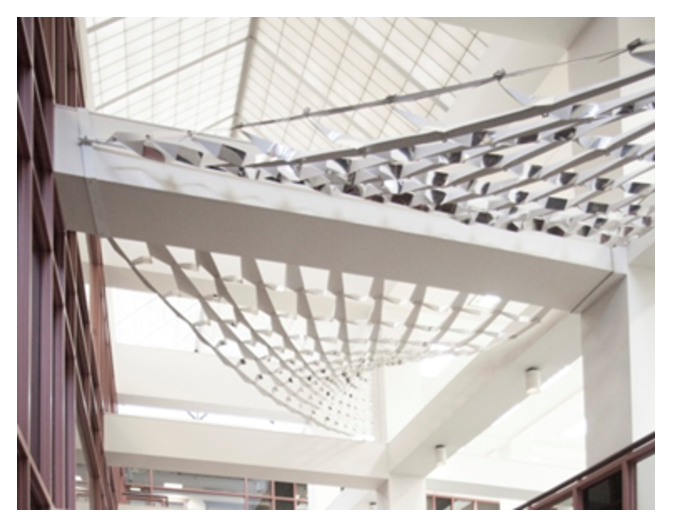
\includegraphics[width=0.6\linewidth]{figures/amp}
\label{fig:amp}}
\qquad \qquad
\subfloat[\mbox{ }]{
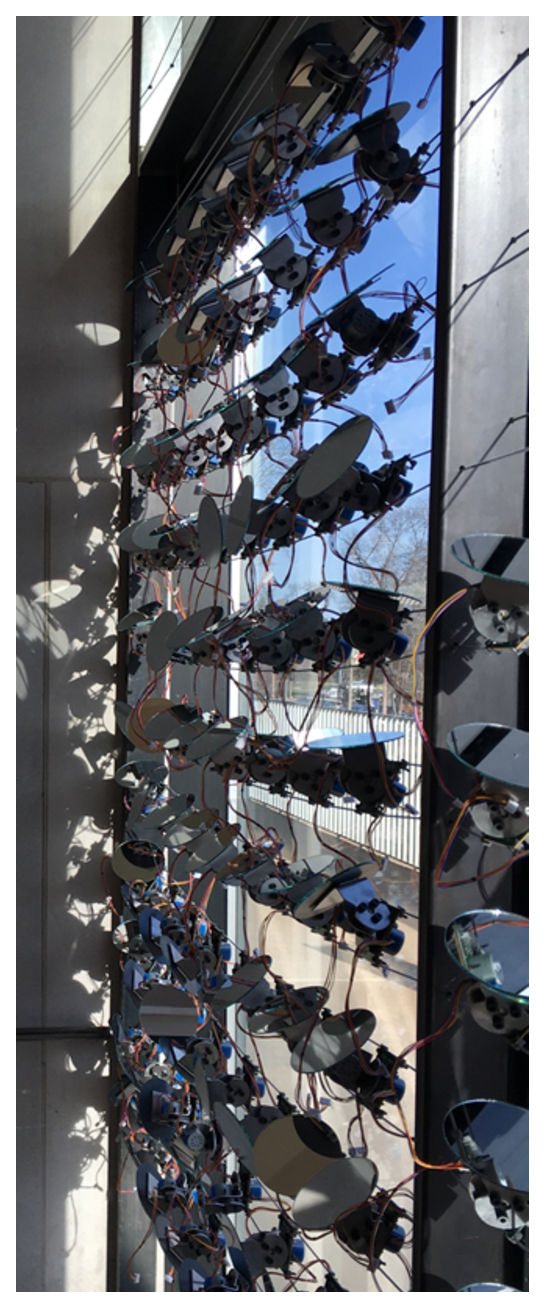
\includegraphics[width=0.19\linewidth]{figures/steinberg}
\label{fig:steinberg}}
\caption{Catoptric system prototypes.
(a)~\emph{AMP}, TRex building, St.~Louis.
(b)~Steinberg Hall, St.~Louis.
}
\label{fig:proto}
\end{figure}

\section{Research Description}
\label{sec:research}

\subsection{CPS Research Focus}

\FIXME{Here, we must ``identify and describe the specific core CPS research
areas being addressed in which novel and foundational research contributions
are being made."}

\subsection{Background and Related Work}
\label{sec:background}

\FIXME{This text is from 2018 proposal and needs to be updated.}

This research proposal builds on ideas, models, and techniques pioneered in two 
previous projects.
The first project, titled \emph{AMP}, created a prototype to redirect
daylight deeper into specific locations with a lightwell.
The building in which the prototype was installed is an 8~story factory
building built in 1895, in which a 5~story light well was cut out of
the floors. A skylight was located above the lightwell and provided the
daylight source.  The primary goal of the project was to develop and use
computational techniques to be able to reflect the rays of light into
the darker recesses of the lightwell. 
Figure~\ref{fig:raytracing} shows an example output from the resulting software
system (analyzing a hypothetical location).
A secondary goal of that work was to develop
a catoptric surface that connected to existing columns and beams, which was
divided into 300 reflective sub-surfaces to achieve the goal.
The project verified that the 300 custom geometrical sub-surfaces
could be designed and fabricated (see Figure~\ref{fig:amp}).
Though successful in its aims, an important limitation of the project
was that each reflective sub-surface had a fixed geometry.

\begin{figure}[ht]
\centering
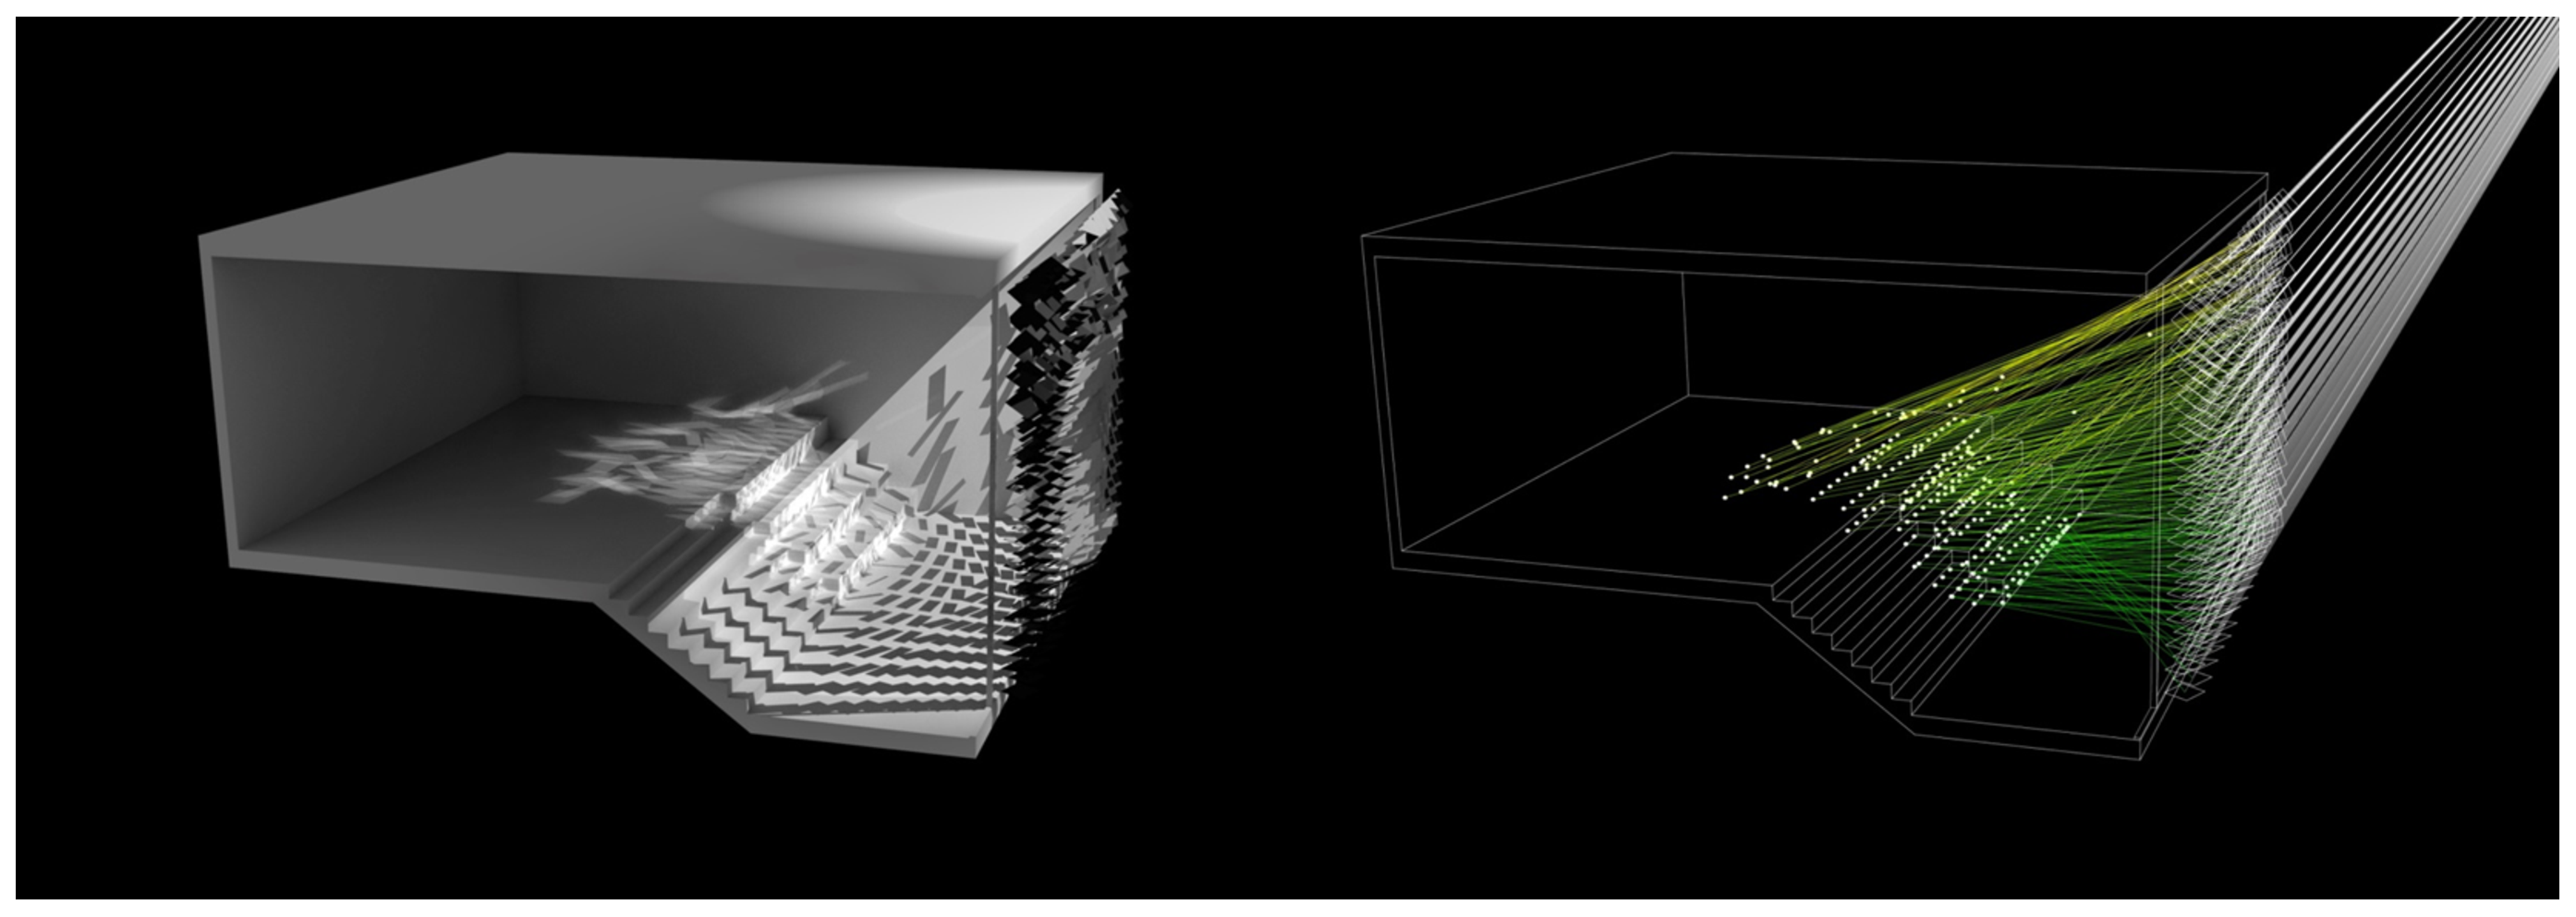
\includegraphics[width=0.95\linewidth]{figures/raytracing}
\caption{Ray tracing analysis of daylighting design.}
\label{fig:raytracing}
\end{figure}

The second project, titled \emph{Catoptric Surface: Steinberg prototype},
addressed that limitation of fixed geometry in AMP. The goal of this second
prototype was to create a series of mirrors that were independently
adjustable according to both the sun's position throughout the day and the desired
location within the building towards which to reflect the light. The ability to
vary the intensity of reflected daylight within the interior of a
building provides the occupants control of the light level for varying tasks
such as a lower light level required to read from a screen versus higher
light level for reading physical paper. This increased level of control
was enabled via the development of units providing 2 axes of rotation of each mirror
independently under software control. This second prototype provides a proof
of concept that individually controlled mirrors can effectively direct
daylight in a very controlled geometry. 
Figure~\ref{fig:steinberg2} shows a CAD illustration of the prototype,
and Figure~\ref{fig:steinberg} shows a photograph of a small number of
the installed mirrors.

\begin{figure}[ht]
\centering
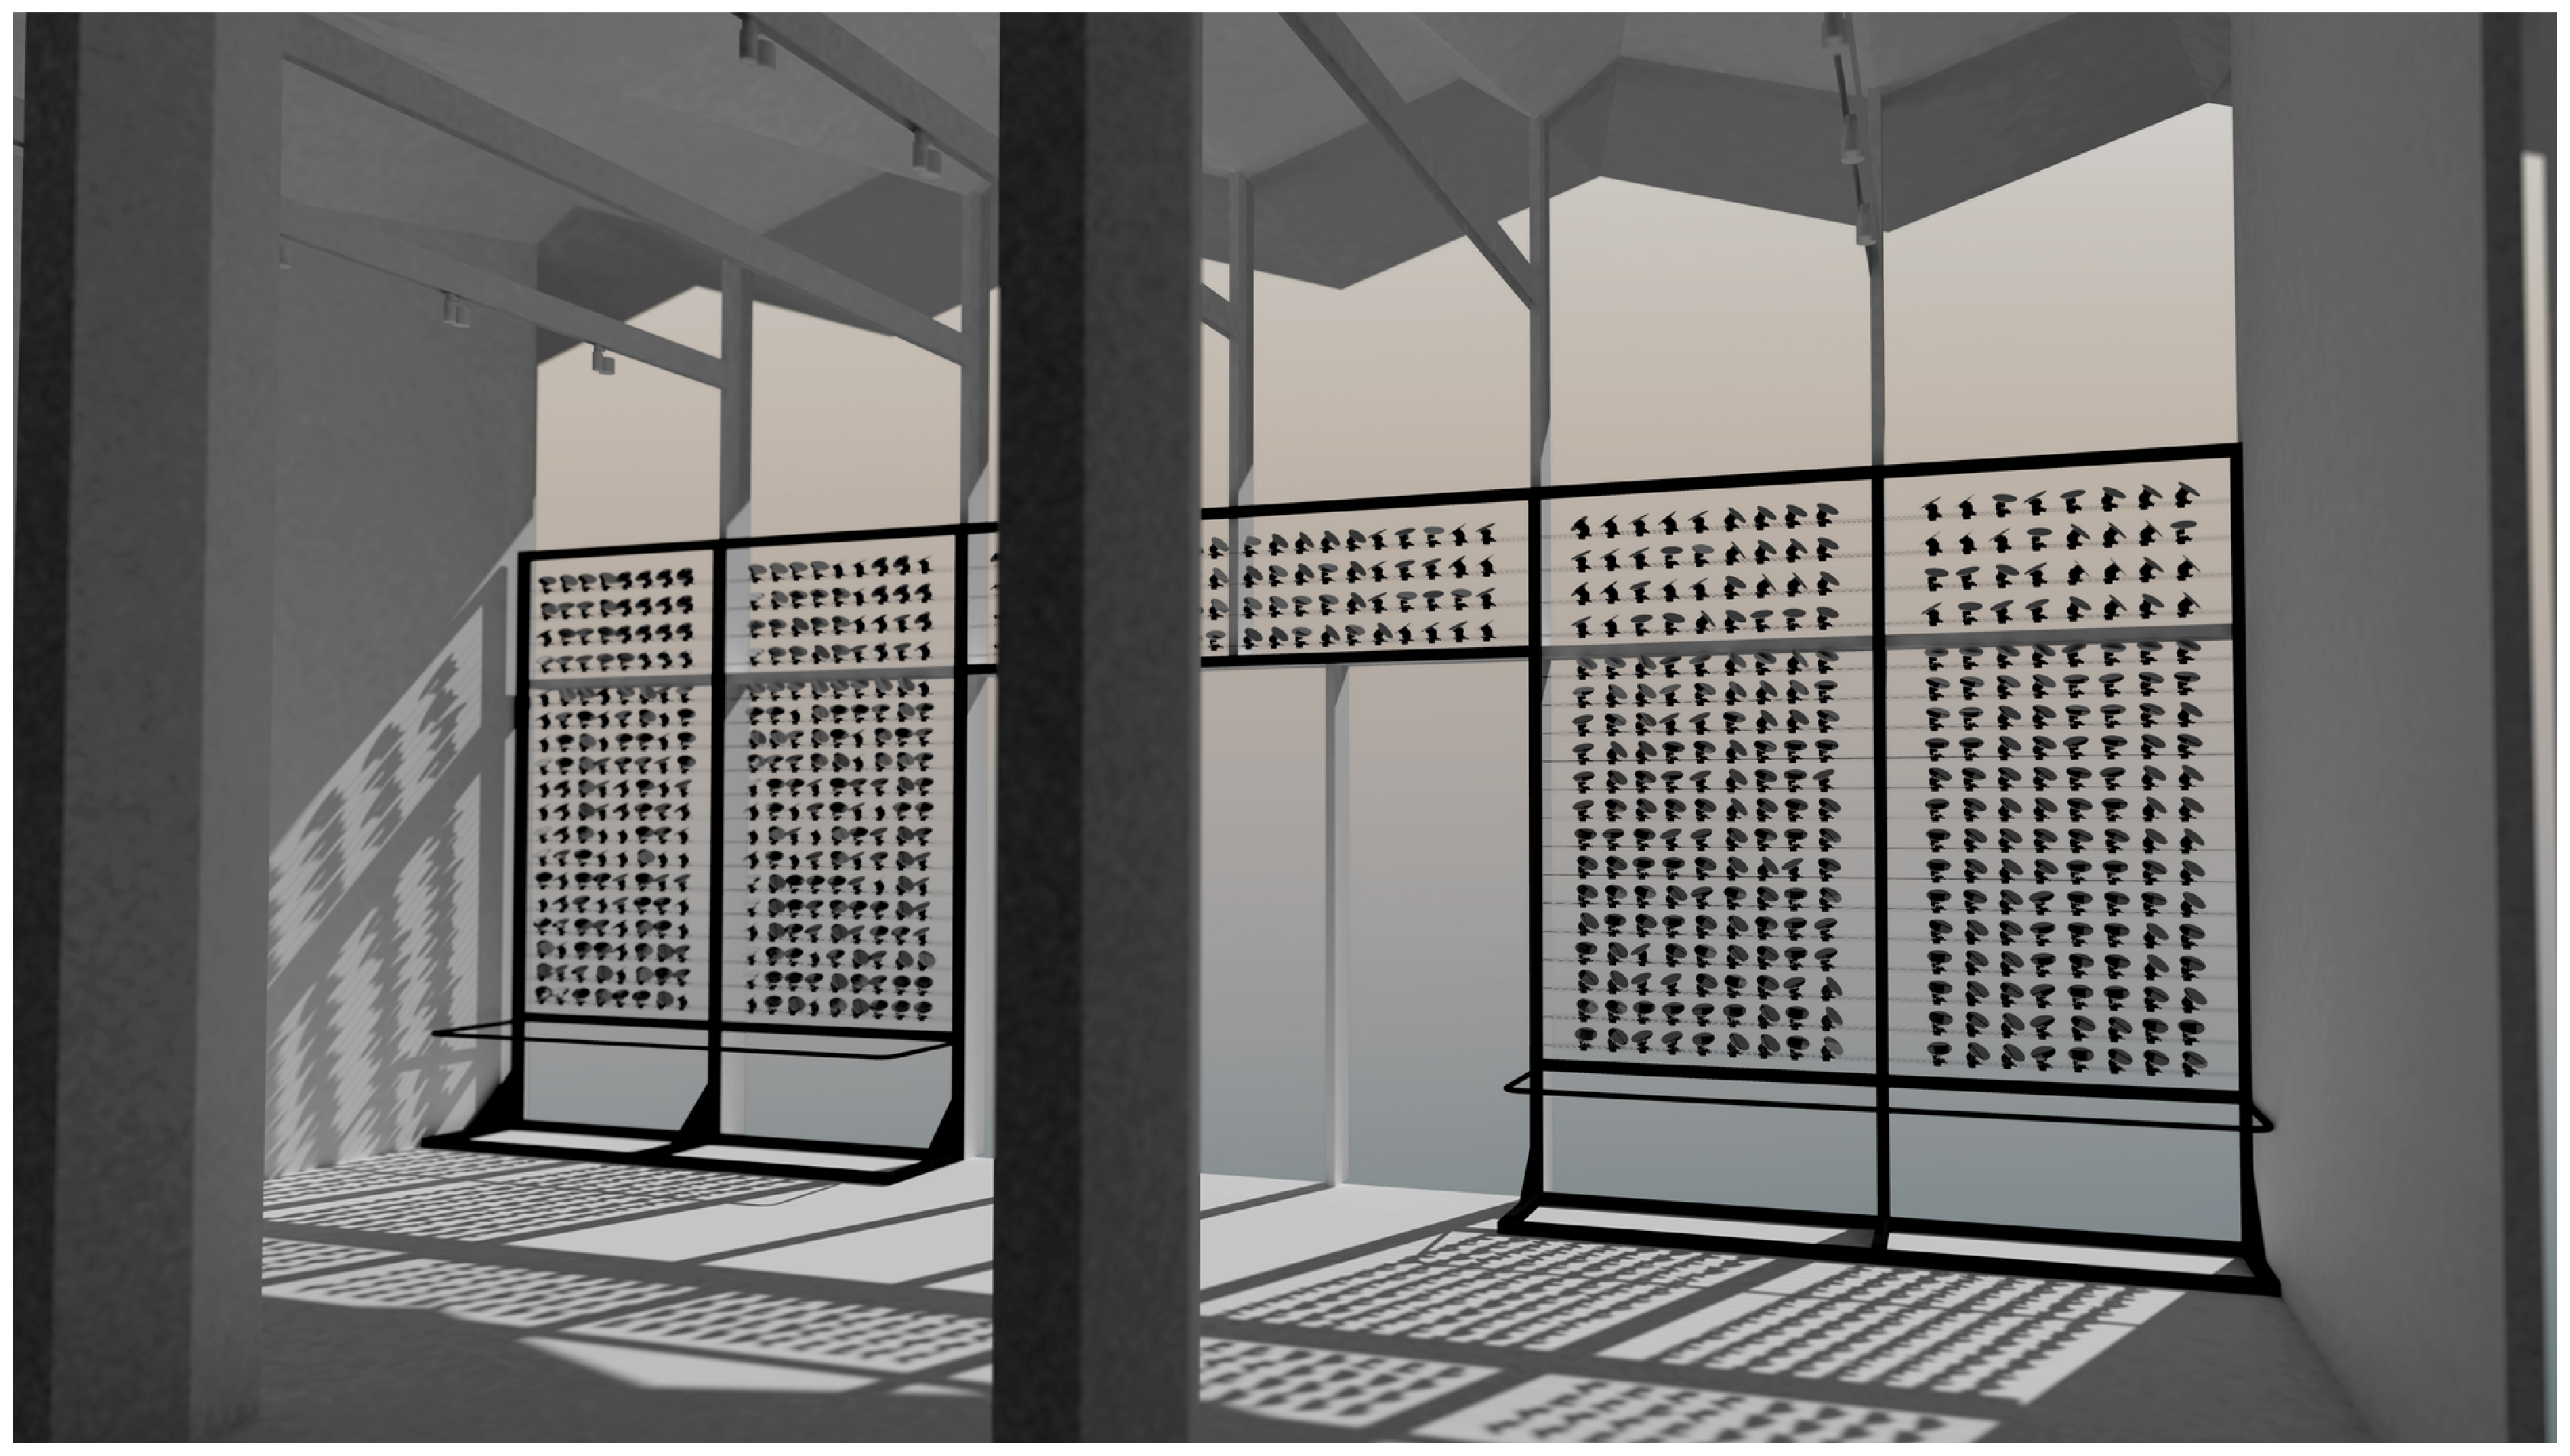
\includegraphics[width=0.9\linewidth]{figures/steinberg2}
\caption{CAD drawing of the Steinberg Hall prototype catoptric surface.}
\label{fig:steinberg2}
\end{figure}

Leslie~\cite{Leslie03} and Alrubaih et al.~\cite{azaise13} provide
a pair of review articles that effectively summarize current
approaches to daylighting in modern building design.
For the most part, these are passive systems, or might include
active control of shades~\cite{kt16}, with a strong emphasis on
achieving uniform, homogeneous illumination~\cite{bwkk15,gb16}.
Our emphasis is on dynamic control of the light position, with the explicit
intent to support inhomogeneous as well as homogeneous illumination patterns.

There have been a number of efforts to quantitatively model, and
empirically measure, prototype daylighting
systems~\cite{bwkk15,fsdm14,ls06,vm16,vgf+13}. A pair of studies, first by
Lee and Selkowitz~\cite{ls06} and followed by Fernandes et al.~\cite{fsdm14},
initially evaluated the potential for energy savings in the New York Times
Headquarters building and then measured the actual realized savings.

In this work, we will exploit Markov Decision Process (MDP)
theory~\cite{puterman} as a formal approach to optimize
catoptric surface control. MDPs represent a general approach
to modeling optimization problems and have been applied in a diverse set of
application areas~\cite{White93}: examples include robotics~\cite{ab10}, 
economics~\cite{bs98}, experiment design~\cite{kb85},
medical decisions~\cite{ahsr10}, manufacturing~\cite{yyl04},
agriculture~\cite{Kristensen03},
and our own group's use in real-time scheduling~\cite{gtsg08,tggs10}
and wireless spectrum management~\cite{mgc16}.

Our prior research has used Markov decision process
models~\cite{gtsg08} to generate resource management policies
off-line~\cite{gtgs09} for non-preemptive sharing of a resource
among multiple purposes at once on-line.  For example, a meter-tall robot's
camera (oriented by a pan-tilt unit similar to the ones we propose to
use in our multi-mirror catoptric installations) may be directed
downward to identify wire-frame chairs and other obstacles to
navigation that other sensors on the robot may have difficulty
detecting, or it may be directed upward to identify faces of people at
a social event whose images it can then capture. Given distributions of
the durations of intervals during which the camera would need to
remain pointed in a given direction to complete an individual task,
standard policy iteration techniques then can be used to generate
run-time policies that in expectation maximize an objective such as
adherence to a strictly proportional allocation of the resource over
time~\cite{gtsg08}, or even a more general definition of the utility 
of completing the different tasks at particular times~\cite{tggs10}.
We also showed that when different distributions of task completion
intervals can occur in different modes (e.g., when a robot moves
from room to room), it is possible to learn on-line what mode
the system is in, or if the mode is known what the distributions are,
but not both~\cite{gtgsuai10}.

However, policy iteration is exponentially expensive in its computational
requirements, and even the memory requirements to store complete policies 
for on-line use may be prohibitive in resource-limited systems.  We 
therefore focused next on the policies that were being generated from 
the models, and discovered consistent structure in those policies that 
allowed a reasonable heuristic approximation.  For simple proportional 
sharing, a single geometric partition of a simplex could be calibrated 
to encode the appropriate policy accurately~\cite{gtspmgs10}.
For utility-based resource sharing multiple disjoint heuristics were needed but
the most effective one to use was clearly defined by problem parameters~\cite{tblwgs11}.

As a further illustration both of the applicability of MDP-based
policy iteration to generate effective resource management policies,
we applied similar techniques to manage another dissimilar resource: 
the transmission spectrum in wireless networks~\cite{mskgct13}.  
Although the semantics of that resource differed radically from the pan-tilt camera, 
the MDP models were reasonably similar.  We extended the basic model to
include modulation as well as admission decisions, discovered and characterized
common structure among the policies that were generated, and again obtained
efficient and effective heuristic policies for on-line use~\cite{mgc16}.

In this proposal we adopt the definition used in our prior work~\cite{gtsg08}
of a (discrete-time) Markov decision process as a 5-tuple
$(\mathcal{X}, \mathcal{A}, T, R, \gamma)$, with \emph{states} designated
as $\chi \in \mathcal{X}$, \emph{actions} designated as $a \in \mathcal{A}$,
and a transition system, $T$, which gives the probability
$P_T (\chi' \mid \chi, a)$ of transitioning from state $\chi$ to
state $\chi'$ on action $a$.
The reward function $R(\chi, a, \chi') \in \mathbb R_{\ge 0}$ describes the
reward that accrues when transitioning from state $\chi$ to
state $\chi'$ via action $a$, under a discount factor, $\gamma$,
to ensure convergence of the long term reward.
In what follows, we will explain how we plan to exploit the formal theory of 
MDPs as an approach to optimization of the configuration of catoptric surfaces.

\subsection{Research Questions}

\subsection{Intellectual Merit}

\FIXME{This section is strictly required. One option is to use it to summarize
the research directions. Another option is to merge it with the section
above, which articulates the research questions we want to address and how
we will go about tackling them. If we do the latter, we must maintain
\emph{this} section title.}

\section{Evaluation/Experimentation Plan}
\label{sec:eval}

\FIXME{Text from 2018 proposal, needs to be updated.}

In this research we will develop, experiment with, and evaluate three prototype 
catoptric surfaces, each installed in a different environment and each with
unique features that will serve to explore different aspects of our approach.
The first prototype is the system currently being installed in the south window 
of Steinberg Hall's atrium (described in Section~\ref{sec:background}).
The second prototype will be designed for and installed at VelociData, Inc.,
a startup firm in St.~Louis that is located in the recently announced \emph{39~North}
innovation district.
The third prototype will be designed for and installed at BECS Technology, Inc.,
a local manufacturer of electronic control systems that has recently
relocated to a newly redeveloped 42,000~sq.~ft. facility. We now discuss each
installation in more detail, followed by a discussion of our software development
and assessment plans.

\subsection{Steinberg Hall, Washington University in St. Louis}

Steinberg Hall is situated on the Danforth Campus of Washington University
in St.~Louis. It is one of the buildings housing the university's College 
of Architecture, and is within easy walking distance of the Dept. of
Computer Science and Engineering.

The catoptric surface that is being installed at the south end of the
atrium will be complete by the start of the proposed research project.
We will use it for a number of purposes in our proposed research:
\begin{enumerate}

\item \emph{Development and calibration of quantitative daylight delivery models.}
We will evaluate the effectiveness of our current ray-tracing software
system in assessing the impact of different configurations of the surface
(i.e., various mirror positions).  Empirical evaluation will use a number
of light meters distributed within the space. The data collected will be
compared to our predictions as well as the analytical models
of both Bueno et al.~\cite{bwkk15} and Galatioto and Beccali~\cite{gb16}.

\item \emph{Practical aspects.}  We expect to learn a number of
  practical things from this installation. By design, these will
  include the positioning precision that is achievable with our
  current physical design, the viability of operating the mirror
  positioning motors open-loop (the pan-tilt is stepper motor driven
  and the current system does not incorporate shaft encoders or other
  positioning feedback), the benefits (if any) of controlling
  acceleration in addition to position, the timing requirements for
  configuration changes, and the ability to effect multiple mirror
  movements in parallel. In addition, we expect to discover new insights
  beyond these anticipated issues, simply through the direct implementation, 
  experimentation, and evaluation of systems.

\item \emph{Investigation of the ability to provide positioning feedback via
image analysis.}  We will install a camera with the full surface in its
field of view and assess the viability of using image analysis techniques
to discern the orientation of each mirror.  An important component of this
investigation will be to quantify the degree of precision that is achievable.

\item \emph{Quantification of the viable heat transfer.}
We will perform a controlled experiment in which we will focus varying
amounts of sunlight on a vessel of water to determine the temperature
rise that is achievable.  This will enable us to calibrate heat transfer
models that will go into the MDP formulation.

\item \emph{Reliability testing of the components.}
This installation is not permanent. When it is decommissioned, we will
setup a representative collection of the mirror components in our laboratory
for stress testing (to failure).  This will allow us to calibrate our
reliability models for inclusion in the MDPs.

\end{enumerate}

\subsection{VelociData, Inc., 39 North Innovation District}

VelociData, Inc., is located at 10425 Old Olive Street Rd., St.~Louis, MO.
They are in the \emph{39 North} innovation district, which has the Danforth
Plant Science Center, Monsanto, Bio Research \& Development Growth Park,
and Heliz Center Biotech Incubator as anchors. It is a 10~min.~drive from
the Washington University Danforth Campus, and they have given us
permission to install a prototype at their facility (see letter
of collaboration).

There are a pair of potential installation sites at VelociData's location:
an east-facing window provides light to an individual's office, and
(the more interesting option) a pair of west-facing windows that provide
light to a bullpen of cubicles occupied by design engineers.
As we will not be able to tie into the HVAC system at this location, our
objectives will be focused on the daylighting benefits, including their
impact on the occupants of the space\footnote{All experimentation that
includes human subjects will undergo review by the Washington University
IRB prior to implementation.}.

We will use this installation for the following purposes:

\begin{enumerate}

\item \emph{Perform safety testing}\footnote{Note: we only operate the Steinberg
surface under active human supervision, as the automated safe operation cannot yet be 
ensured.}.
We will perform stress testing on the installed system, injecting errors so as to
intentionally attempt to create unsafe conditions, all the while monitoring
to ensure that safety is maintained.

\item \emph{Assess utility of non-southern facing windows.}
Since the windows at VelociData's location are on the top floor, and face
either east or west, this gives us the opportunity to explore the viability
of exploiting multiple-reflection designs
(e.g., a fixed position mirror above the
roofline that redirects sunlight to the active catoptric surface).

\item \emph{Evaluate human responses.}
While we do not have the budget in this project to perform
comprehensive productivity analyses, we will be in a position to
query the building occupants about their experience with the
daylight effects. E.g., do they see value in the controllability
of the quantity of daylight?

\item \emph{Iterate to refine the design.}
As these are prototype systems, we have no expectation that the
initial versions will operate entirely as desired.  We will redesign
and rebuild as needed to make progress on the research questions we
are investigating.

\end{enumerate}

\subsection{BECS Technology, Inc., St. Louis County}

BECS Technology, Inc., is located at
10818~Midwest Industrial Dr., St.~Louis, MO.
They are a small manufacturer of electronic control
systems for a number of markets (e.g., agriculture, aquatics, refrigeration).
The unique benefit to this installation is that they have agreed to
allow us to have access to the HVAC system in their building (see letter
of collaboration).

The HVAC system at BECS is one in which the hydronic water loop
also serves as the fire protection sprinkler system~\cite{Janus01,wm79}.
Individual heat exchangers either deliver heat into the loop 
(e.g., from a boiler) or extract heat from the loop (e.g., to a
cooling tower).
An experimental loop that can be the focus point for light from
a catoptric surface can be readily incorporated into a system such
as this.  The integration is made even easier because BECS, as
a manufacturer of aquatics equipment, uses a controller of its own
design to manage the entire system.

We will use this installation for the following purposes:

\begin{enumerate}

\item \emph{Repeat assessments from initial installations.}
As each installation will have a unique configuration, we will exploit the
latter two installations (at VelociData and BECS) to perform common
experiments at each, comparing the results to increase the confidence
in any conclusions that we draw based on empirical data.
This will include all of the calibration efforts, as well as the comparison
of empirical data to the theoretical models (both for daylight delivery
and thermal heat transfer).
This will also include any human evaluations that are undertaken at
the VelociData site.

\item \emph{Integration into the HVAC system.}
We will implement a heating loop that is capable of delivering
thermal energy into the building's main hydronic water loop.
The temperature of the water in this loop will be logged, and the
master HVAC controller (built by BECS) will enable us to determine
the effectiveness of the heat transfer.  We will also be able to
quantify the amount of energy savings that results.

\item \emph{Assessment of manufacturability.}
As described in the Transfer to Practice Supplementary Document, BECS
is planning to assist us in evaluating the commercial viability of the
catoptric surface as a product.  An important piece of this evaluation is
the assessment (by design and manufacturing engineers at BECS) of the
manufacturability of the system.

\item \emph{Iterate to refine the design.} Again, we do not expect the initial design
to be all that it can be. As for the previous systems, we will redesign
and rebuild as needed.

\end{enumerate}

\subsection{Software Development and Assessment}

The current software for raytracing and physical modeling is within
Rhinoceros 3D (Rhino3D), a free form surface modeling system that utilizes a
non-uniform rational B-spline (NURBS) mathematical representation.
The current optimization (not MDP-based) is coded using
Grasshopper, a visual programming language plug-in.
Grasshopper has been used in the past for lighting performance
analysis~\cite{Echarri16,Willis16}.

The existing positioning software is written in a combination of
Python (executing on a Raspberry Pi) and C (executing on an Arduino Uno).
The Rhino3D/Grasshopper output is made available to the Python code via CSV
files in the filesystem.

The existing MDP model software is written in C++ and currently is not integrated
into the above software components at all.
Clearly, an important software development task in this research project
will be to enable each of the above software elements to interact with one
another, preferably in a relatively seamless manner, aided by modern compilers'
and iterpreters' ability to integrate code written in multiple programming
languages.

When our research group develops software that is intended to support
the research questions being investigated (as opposed to the software
effort being the research question itself), we have a practice of adopting
software engineering techniques that closely approximate those used
in industrial settings.  For example, we have regular code reviews,
testing is performed by individuals who are distinct from the developers,
the software design is presented to the group and its pros and cons
discussed prior to implementation, etc.

The assessment of the software will primarily be embodied in the evaluation
of the catoptric surfaces themselves.  However, we will evaluate the
performance of all of the software, ensuring that execution times are
reasonable for off-line tasks and deadlines are met for real-time tasks.
All software developed in this proposed research will be released as open-source,
and in addition to making the code freely available on the web we will provide
specific mechanisms for the broader research community to interact with our
team to provide feedback, request enhancements, and otherwise engage with
us as we conduct this research.

\section{Project Management and Collaboration Plan}
\label{sec:collab}

\FIXME{Text from 2018 proposal, needs to be updated.}

We first describe the investigator team, including each of our primary roles
in the project.  This is followed by a description of our approach
to collaboration and a timeline for the research activities.

{\bf Roger D. Chamberlain}, PI, is a Professor of Computer Science
and Engineering in the School of Engineering and Applied Science
at Washington University in St.~Louis.
Prof.~Chamberlain will have overall responsibility for managing the
research project and will take the lead in development of Markov
decision process models, performance evaluation, and electrical engineering
design requirements.

{\bf Chandler Ahrens}, Co-PI, is an Associate Professor of Architecture
in the Sam Fox School of Design \& Visual Arts at Washington University in St.~Louis.
Prof.~Ahrens will take the lead in the physical design aspects of
the catoptric surfaces, including their shape, configuration, positioning,
fabrication, and installation.

{\bf Chris Gill}, Co-PI, is a Professor of Computer Science
and Engineering in the School of Engineering and Applied Science
at Washington University in St.~Louis.
Prof.~Gill will lead the software development efforts, with an emphasis
on design for reuse whenever reasonable.  He will also lead our
approach to reusable abstractions that can be generalized to other
cyber-physical system uses.

All three faculty have worked together in different combinations in the 
past, so the organization and management of the present collaboration 
will be straightforward.  Existing publications co-authored by two or 
more of the investigators include~\cite{acmb18,cag18,cagm18,mgc16, mskgct13}.
Ahrens 
and Chamberlain collaborated on the design and implementation of the 
catoptric surface being installed in Steinberg Hall, and Chamberlain 
and Gill have previously co-advised a doctoral student (J.~Meier, 
PhD, currently at Lockheed Martin) who exploited Markov decision 
processes for RF spectrum management.

We will exploit the fact that the entire team is located on the
Danforth Campus of Washington University in St.~Louis to organize
our collaborations around regular (weekly) face-to-face meetings.  
These meetings will form the backbone of the collaboration, where 
we check in with each other to update status, plan next steps, and 
address any issues that have arisen since our previous meeting.
In addition to these regular checkpoints, the investigators and
students involved in the project will meet in different combinations
as appropriate during each week, throughout the conduct of the 
proposed research.

We will also gather for the purpose of reviewing the literature
(traditional journal club activities, which CSE doctoral students
are required to take during their PhD programs), student 
presentations (frequently practice talks for upcoming conference 
and student seminar presentations), and reports to the group from 
anyone who has recently returned from a conference trip.

Our initial plan for the project timeline is listed below, indicating the
primary activities to be pursued in each year of the project.

\subsection*{Year 1}

\begin{itemize}

\item Perform quantitative measurements using the Steinberg catoptric surface.

\item Design initial MDPs, incorporating daylighting and heat harvesting.

\item Develop initial abstractions for low-level controller software.

\item Evaluate imaging approach for positioning feedback.

\item Perform initial design work for VelociData installation.

\item Submit human subjects evaluation plan to IRB for approval.

\end{itemize}

\subsection*{Year 2}

\begin{itemize}

\item Decommission the Steinberg surface and re-purpose components for
reliability testing.

\item Expand MDPs to include additional constraints (i.e., to ensure
safety).

\item Develop initial abstractions for MDP-based optimization software.

\item Install VelociData catoptric surface and perform empirical evaluation.

\item Perform quality of experience evaluation for VelociData users.

\item Perform initial design work for BECS installation.

\end{itemize}

\subsection*{Year 3}

\begin{itemize}

\item Expand MDPs to include additional goals (e.g., to prioritize
reliability).

\item Install BECS catoptric surface and perform empirical evaluation.

\item Perform quality of experience evaluation for BECS users.

\item Refine software abstractions for both low-level positioning control
and high-level MDP-based optimization, based upon what has been learned
from earlier editions.

\item Release software under open source licensing terms.

\end{itemize}

\section{Broader Impacts}
\label{sec:broader}

\FIXME{Text from 2018 proposal, needs to be updated.}

The proposed research is expected to have important impacts on the built environment.
According to the EPA, buildings are responsible for producing 6\% of
greenhouse gasses and heat and electrical generation produces another
25\%\footnote{\url{https://www.epa.gov/ghgemissions/global-greenhouse-gas-emissions-data}}.
A large portion of the electrical consumption in buildings is used for
heating, cooling and artificial lighting. Our proposal addresses the
reduction of electricity for artificial lighting to be replaced by
reflected daylight and capturing the solar heat. During daytime hours,
daylight is a preferred source of light for many people and the proposal
directs the daylight deeper into a building. The daylight reflection system
provides a more sustainable approach by reducing the required electricity
and provides a more desirable quality of light.

At the undergraduate level, this work is closely related to
our second-semester introductory course in computer science and
computer engineering.  The
text (co-authored by PI R. Chamberlain) is entitled {\it Computing
in the Physical World}~\cite{cc17}, and the course provides an introduction to
cyber-physical systems concepts in a laboratory-based setting.

The computational platform used in the course (an Arduino Uno) is the
same one used to control the Steinberg prototype catoptric surface,
and it has a very large hobbyist following (in the maker community).
We regularly request support for Research Experience for Undergraduate
(REU) students, and individuals who have completed
the above course will be well prepared to contribute to the research.

At the graduate education level, this work will support 4 graduate
students at Washington Univ.~in St.~Louis.
These students will be some combination of engineering students and
architecture students, with each community of students learning from
the other to broaden their individual horizons of experience to
include multidisciplinary work.

The Steinberg prototype was substantially designed by a student pursuing
dual degrees in architecture (MArch) and engineering (MEng)~\cite{Mitchell18}.
He recently gave an invited presentation to the Washington University Board
of Trustees about his experience, and the university is considering
a broader set of educational offerings that are tailored to students with
similar, cross-disciplinary interests.

We will leverage a pair of existing university programs to help us
attract students from traditionally underrepresented groups.  The Olin
Fellowship Program (for women) and the Chancellor's Fellowship Program
(aimed to recruit, support, and retain underrepresented minority 
students) have a successful track
record of enabling individuals to pursue graduate study.  In our
experience, the most effective method for attracting students from
underrepresented groups is by personal contact with a suitable role
model.  To facilitate this, we regularly ask the appropriately
qualified individuals in our group to be actively involved in the
recruiting process.  This cohort currently includes two
minority graduate students (one African-American student and one Hispanic 
student).
We will attempt to leverage the maker space community as one target
for broadening participation from traditionally underrepresented groups.

\section{Results from Prior NSF Support}
\label{sec:prior}

Co-PI C. Ahrens has not had prior NSF funding. The projects described
below are representative examples of NSF-supported research led by PI 
R.~Chamberlain and co-PI C.~Gill.

\noindent
{\large\bf CSR: Small: Concurrent Accelerated Data Integration}
{\bf (CNS-1527510,
PI R. Chamberlain, co-PI Ron Cytron)}, 
10/2015--9/2019, \$519,275.  

\textbf{Intellectual Merit} -- This ongoing project is investigating the
accelerated execution of data integration workflows, which
increasingly are bottlenecks in data science. Execution platforms
being targeted include both graphics engines and FPGAs.

\textbf{Broader Impacts} -- This research project has supported 3
graduate students and 4 REU students.  The applications investigated
come from the fields of computational biology, astrophysics, and the
Internet of Things, further expanding the scope of the students'
experience.

\textbf{Evidence of Research Products and their Availability} --
Publications resulting from this work include~\cite{dibs,c17,mgc16,js16}.
A benchmark suite of the above workflows has been released
as a community resource~\cite{dibsv1}.

\noindent
{\large\bf CPS: Medium: Collaborative: CyberMech, a Novel Run-Time Substrate for 
Cyber-Mechanical Systems}
{\bf (CNS-1136073 and CNS-1136075,
Washington University: PI C. Gill, co-PIs Kunal Agrawal and Chenyang Lu; Purdue University: PI Arun Prakash, co-PI Shirley Dyke)}, 9/2011-8/2016, \$1,800,000 total.  

This research project developed novel foundations for parallel real-time computing, and used them to demonstrate the first ever real-time hybrid simulation involving a thousand-degree-of-freedom structure at millisecond time scales.

\textbf{Intellectual Merit} -- Results of this research include new methods for parallel real-time execution of control and simulation computations, new parallel real-time scheduling techniques and analyses, and characterization and exploitation of trade-offs involving both high computational demand and stringent timing constraints.

\textbf{Broader Impacts} -- This multi-university project involved 7 PhD, 3 masters, and 7 undergraduate students, and 2 visiting scholars in highly multi-disciplinary research collaborations.  Results of this research are spurring discussions on scalability of real-time hybrid simulation techniques, at workshops on topics of current interest in the earthquake engineering research community, including at a recent NSF-sponsored workshop at UCSD on multi-hazard engineering.

\textbf{Evidence of Research Products and their Availability} -- Results of this 
collaborative research appeared in 10 publications at top-tier conferences and journals.
Data, experiment configurations, platform software, and simulation source-code 
have been published on-line at Washington University and Purdue University.


%\input{conclude}

\clearpage
% \begin{scriptsize}
\bibliographystyle{abbrv}
\bibliography{prop}
% \end{scriptsize}

\end{document}
